%; whizzy paragraph -pdf xpdf -latex ./whizzypdfptex.sh
%; whizzy-paragraph "^\\\\begin{frame}\\|\\\\emtext"
% latex beamer presentation.
% platex, latex-beamer でコンパイルすることを想定。 

%     Tokyo Debian Meeting resources
%     Copyright (C) 2012 Junichi Uekawa
%     Copyright (C) 2016 Nobuhiro Iwamatsu

%     This program is free software; you can redistribute it and/or modify
%     it under the terms of the GNU General Public License as published by
%     the Free Software Foundation; either version 2 of the License, or
%     (at your option) any later version.

%     This program is distributed in the hope that it will be useful,
%     but WITHOUT ANY WARRANTY; without even the implied warreanty of
%     MERCHANTABILITY or FITNESS FOR A PARTICULAR PURPOSE.  See the
%     GNU General Public License for more details.

%     You should have received a copy of the GNU General Public License
%     along with this program; if not, write to the Free Software
%     Foundation, Inc., 51 Franklin St, Fifth Floor, Boston, MA  02110-1301 USA

\documentclass[cjk,dvipdfmx,12pt]{beamer}
\usetheme{Tokyo}
\usepackage{monthlypresentation}

%  preview (shell-command (concat "evince " (replace-regexp-in-string "tex$" "pdf"(buffer-file-name)) "&")) 
%  presentation (shell-command (concat "xpdf -fullscreen " (replace-regexp-in-string "tex$" "pdf"(buffer-file-name)) "&"))
%  presentation (shell-command (concat "evince " (replace-regexp-in-string "tex$" "pdf"(buffer-file-name)) "&"))

%http://www.naney.org/diki/dk/hyperref.html
%日本語EUC系環境の時
\AtBeginDvi{\special{pdf:tounicode EUC-UCS2}}
%シフトJIS系環境の時
%\AtBeginDvi{\special{pdf:tounicode 90ms-RKSJ-UCS2}}

\newenvironment{commandlinesmall}%
{\VerbatimEnvironment
  \begin{Sbox}\begin{minipage}{1.0\hsize}\begin{fontsize}{8}{8} \begin{BVerbatim}}%
{\end{BVerbatim}\end{fontsize}\end{minipage}\end{Sbox}
  \setlength{\fboxsep}{8pt}
% start on a new paragraph

\vspace{6pt}% skip before
\fcolorbox{dancerdarkblue}{dancerlightblue}{\TheSbox}

\vspace{6pt}% skip after
}
%end of commandlinesmall

\title{Debian Update}
\subtitle{OSC 2019 Tokyo/Fall \\東京エリアDebian勉強会(出張版)}
\author{Debian JP Project \\杉本 典充\\ dictoss@debian.or.jp}
\date{2019年11月23日}
\logo{
\includegraphics[width=8cm]{image200607/openlogo-light.eps}}

\begin{document}

%-------------------

\section{表紙}

\begin{frame}
\titlepage{}
\end{frame}

\section{目次}

\begin{frame}{Agenda}
  \begin{itemize}
  \item Debian とは?
  \item Debian JP Project と Debian 勉強会
  \item Debian 10 (buster)
  \item Debian Updates
  \item 今後のイベント
  \end{itemize}
\end{frame}

%-------------------

\section{Debian とは?}

\begin{frame}
  \begin{center}\Huge{Debian とは?}\end{center}
\end{frame}


\begin{frame}{Debian とは?}

{\color{red}{フリー/オープン}}な{\color{red}{ユニバーサル}}オペレーティングシステム を作成しようとするボランティアベースのプロジェクト

\begin{table}[htb]
  \begin{tabular}{|c|c|c|}
    \hline
    ディストリ & 企業 & ボランティア \\ \hline
    Fedora & RedHat支援あり & あり  \\ \hline
    RHEL & RedHat & なし  \\ \hline
    CentOS & RedHat支援あり & あり \\ \hline
    \color{red}{Debian}  & \color{red}{なし} & \color{red}{あり} \\ \hline
    Ubuntu  & Canonical & あり \\ \hline
    openSUSE & SUSE支援あり & あり \\ \hline
    SLES & SUSE & なし \\ \hline
  \end{tabular}
\end{table}

\end{frame}

\begin{frame}{Debian とは?}

\begin{itemize}
\item 世界規模で開発が行われている
%\item アップストリームファーストな考え方
\item 公式の Debian 開発者(Debian Developer)は、63ヶ国に約1000名
\item パッケージメンテナや翻訳などの貢献者も入れるともっと多くの人たちが参加
\end{itemize}
  
\end{frame}


\begin{frame}{Debian とは?}

\begin{itemize}
\item 様々な用途に使える汎用的な作り
  \begin{itemize}
  \item デスクトップPC、ノートPCなどの普段利用するコンピュータのOS
  \item Linuxサーバ
    \begin{itemize}
    \item 例:webサーバのシェア:\url{https://w3techs.com/technologies/details/os-linux/all/all})
    \end{itemize}
  \item 組込デバイスのベースOS (多くのCPUで動作する)
  \end{itemize}
\item 「Debian」ベースな派生OSの源流
  \begin{itemize}
  \item 例:Ubuntu、Raspbian、Kali Linux
    % https://debian-handbook.info/browse/en-US/stable/sect.kali.html
  \item 派生先のディストリビューションと相互に情報交換をして開発している
  \end{itemize}
\end{itemize}

\end{frame}


\begin{frame}{Debian とは?}

  \begin{itemize}
  \item 2019年11月の時点で、最新版は {\color{red}{Debian 10.2}} (コードネーム: buster)
    \begin{itemize}
    % https://www.debian.org/releases/buster/amd64/release-notes/ch-whats-new.ja.html
    \item パッケージ数は {\color{red}{約57,000}} 以上を提供
    \item 公式にサポートするCPUアーキテクチャは {\color{red}{10}}
    \end{itemize}\
  \item コードネームはトイ・ストーリーのキャラクター名を採用
  \item 次のメジャーリリース は Debian 11 (コードネーム: {\color{red}{}}bullseye)
    \begin{itemize}
    \item 2021年中頃にリリースすると思われる
    \end{itemize}
\end{itemize}

\end{frame}


\begin{frame}{Debian とは?}

\frametitle{リリースサイクル}
\begin{itemize}
\item リリースサイクル:おおよそ2年
  \begin{itemize}
  \item Debian は time-based freeze を採用
  \end{itemize}
\item 標準サポート期間:3年
\item LTS(Long Term Support):標準サポート期間終了後から 2年
  \begin{itemize}
  \item サポートするアーキテクチャが amd64、i386、arm 系に絞られる
  \item 全パッケージをサポートするわけではなく、主要なパッケージに絞ってサポート
  %\item スポンサーとして資金援助するとメンテナンスするパッケージの希望を出せる
  \end{itemize}
\end{itemize}

\end{frame}


\begin{frame}{Debian Project における理念やルール}

\begin{itemize}
\item Debian 社会契約
  \begin{itemize}
  \item Debian 開発者 たちが目指すフリーソフトウェアコミュニティーの在り方
  \end{itemize}
\item Debian フリーソフトウェアガイドライン(DFSG)
  \begin{itemize}
  \item Debian 社会契約の一部
  \item Debian が考えるフリーソフトウェアの定義
  \item オープンソースの定義のひな形にもなっている
  \end{itemize}
\item Debian Policy
  \begin{itemize}
  \item \url{https://www.debian.org/doc/debian-policy/}
  \item Debian パッケージの区分、内容、ルール、ファイル配置の方針などの技術的な定義
  \end{itemize}
\end{itemize}

\end{frame}


\begin{frame}{DebConf}%[containsverbatim]

\begin{itemize}
\item 年に一回、Debian 開発者が集まって開催するカンファレンス
  \begin{itemize}
  \item 2019/07/21 - 07/28: Debconf19: CURITIBA - BRAZIL
  \item 2020/08/23 - 08/29: Debconf20: Haifa - Israel
  \end{itemize}
\end{itemize}

\begin{center}
  %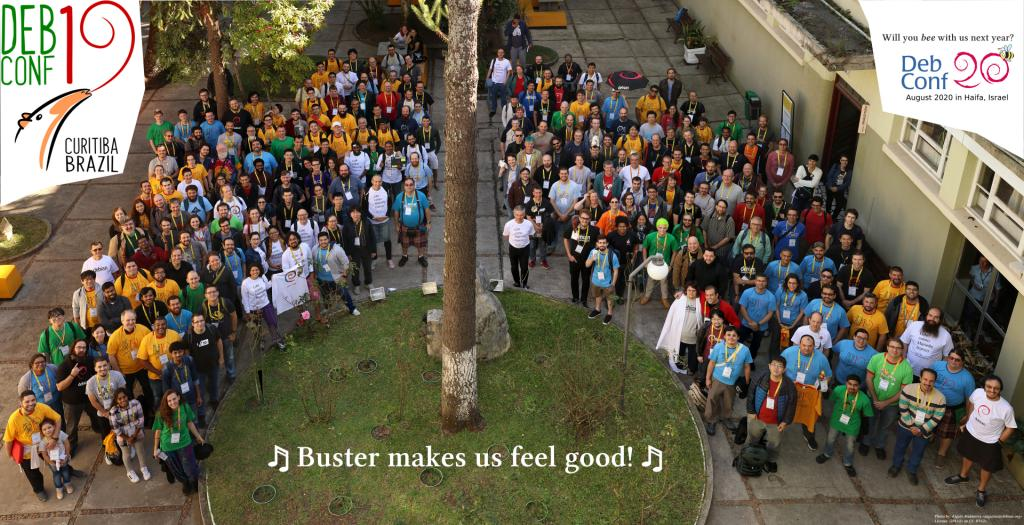
\includegraphics[scale=0.2]{image201911-kansai/debconf19_group_small.jpg}
  %% https://salsa.debian.org/debconf-team/public/share/debconf19/blob/master/photos/aigarius/group/debconf19_group_small.jpg
\end{center}

\end{frame}


\begin{frame}{Debian とは?}
  
まとめると「Debian」とは

\begin{itemize}
  \item フリー/オープンなオペレーティングシステム (OS)を作成しようとする人たちが集まるボランティアベースのプロジェクト
  \item 自分たちの考えるフリーという言葉に関する定義、開発目的、パッケージングポリシーを厳格に決めている
  \item 世界中に1000人以上の開発者がおり、他のディストリビューションのベースとして採用されている
  \item 約2年毎にリリースが行われ、多くのパッケージとアーキテクチャをサポートしている
  \item 上記のような特徴から様々なところで利用されているLinuxディストリビューション
\end{itemize}

\end{frame}

%------------------


\section{Debian JP Project と Debian勉強会}


\begin{frame}
  \begin{center}\Huge{Debian JP Project\\と\\Debian勉強会}\end{center}
\end{frame}

\subsection{Debian JP Projectとは}
  
\begin{frame}{Debian JP Project とは?}

\begin{itemize}
  \item 日本においてDebianを普及させることを目的とした任意団体
  \item 活動内容
  \begin{itemize}
    \item Debian の日本語による情報発信
    \item ユーザとの情報交換
    \item Debian 開発者やパッケージメンテナの育成など
  \end{itemize}
\end{itemize}

\end{frame}

\subsection{Debian勉強会}

\begin{frame}
  
\frametitle{Debian勉強会}
\begin{itemize}
 \item 2005年1月開始
 \item Debian 開発者 上川さんが発起人
 \item 東京と関西で月に一回コンスタントに開催しているDebian 開発者、Debian ユーザによる勉強会
   \begin{itemize}
   \item 東京エリアDebian勉強会
     \begin{itemize}
     \item \url{https://tokyodebian-team.pages.debian.net/}
     \end{itemize}
   \item 関西Debian勉強会
     \begin{itemize}
     \item \url{https://wiki.debian.org/KansaiDebian}
     \end{itemize}
   \end{itemize}
\end{itemize}

\end{frame}


\begin{frame}

\frametitle{Debian勉強会:解決したい内容}
\begin{itemize}
 \item 問題
   \begin{itemize}
   \item MLとIRCで情報交換していた
   \item face-to-faceで合う場所がない
   \item まとまったドキュメントが出てこない
   \end{itemize}
 \item Debian勉強会の提案
   \begin{itemize}
   \item 定期的に集まる
   \item 資料を作成して公開(GPL-2+) \\
	 {\small \url{https://salsa.debian.org/tokyodebian-team/monthly-report}}
   \end{itemize}
\end{itemize}

\end{frame}


\subsection{最近の勉強会}


\begin{frame}
  
\frametitle{Debian勉強会:最近の勉強会}
  
\begin{itemize}
\item 勉強会の内容
  \begin{itemize}
  \item Debian 界隈やパッケージング関連の話題など専門の人に話を聞く
  \item Debianで気になった事柄を調べてレポートする
  \end{itemize}
\item 前回の内容(東京 10月):
  \begin{itemize}
  \item 場所: 荒川区立町屋文化センター
  \item Debian GNU/kFreeBSD セットアップガイド 2019年版
  \item 月間 Debian Policy
  \end{itemize}
\item 各地のイベントでDebian普及活動
  \begin{itemize}
  \item OSC2019北海道、OSC2019京都、OSC2019東京
  \item 関西オープンフォーラム
  \item Debian/Ubuntu ユーザミートアップ in 札幌
  \end{itemize}
\end{itemize}

\end{frame}

%-----------------------

\section{Debian 10 buster}

\begin{frame}
  \begin{center}\Huge{Debian 10 buster\\リリースおめでとう!}\end{center}
\end{frame}


\begin{frame}{Debian 10 buster}% [containsverbatim]

Debian 10 (コードネーム:buster)

\begin{itemize}
\item 2019年7月6日にリリース
\item 最新版は 2019年11月16日 にリリースした Debian 10.2
\end{itemize}

%\begin{center}
  %\includegraphics[width=0.6\hsize]{image201902/buster.jpg}
  % https://pixar.fandom.com/wiki/Buster
%\end{center}

\end{frame}


\subsection{CPUアーキテクチャ}

\begin{frame}{Debian 10 buster}% [containsverbatim]

CPUアーキテクチャ

\begin{itemize}
\item amd64、i386
\item arm64、armel、armhf
\item mips64el、mipsel、mips
\item ppc64el
\item s390x
\end{itemize}
    
\end{frame}


\subsection{提供するソフトウェア}

\begin{frame}{Debian 10 buster}% [containsverbatim]

提供するソフトウェア(1)

\begin{multicols}{2}

  \begin{table}[htb]
    \begin{tabular}{|c|c|}
      \hline
      Linux kernel & 4.19 \\ \hline
      GNOME & 3.30 \\ \hline
      KDE Plasma & 5.14 \\ \hline
      Cinnamon & 3.8.8 \\ \hline
      LXDE & 10 \\ \hline
      LXQt & 0.14 \\ \hline
      MATE & 1.20 \\ \hline
      Xfce & 4.12 \\ \hline
      Chromium & 78.0 \\ \hline
      Firefox ESR & 68 \\ \hline
      Thunderbird & 68 \\ \hline
    \end{tabular}
  \end{table}

  \newpage

  \begin{table}[htb]
    \begin{tabular}{|c|c|}
      \hline
      LibreOffice & 6.1 \\ \hline
      GIMP & 2.10.8 \\ \hline
      Inkscape & 0.92.4 \\ \hline
      MariaDB & 10.3 \\ \hline
      PostgreSQL & 11 \\ \hline
      sqlite & \begin{tabular}{c} 3.27.2 \\ 2.8.17 \end{tabular} \\ \hline
      Emacs & 26.1 \\ \hline
      Vim & 8.1 \\ \hline
      OpenSSH & 7.9p1 \\ \hline
      OpenSSL & 1.1.1d \\ \hline
      GnuPG & \begin{tabular}{c} 2.2.12 \\ 1.4.23\end{tabular} \\ \hline
    \end{tabular}
  \end{table}

\end{multicols}

\end{frame}


\begin{frame}{Debian 10 buster}% [containsverbatim]

提供するソフトウェア(2)

\begin{multicols}{2}

  \begin{table}[htb]
    \begin{tabular}{|c|c|}
      \hline
      Perl & 5.28.1 \\ \hline
      Python & \begin{tabular}{c} 3.7.3 \\ 2.7.16 \end{tabular} \\ \hline
      Ruby & 2.5.1 \\ \hline
      PHP & 7.3 \\ \hline
      Go & 1.11 \\ \hline
      OpenJDK & 11 \\ \hline
      Rustc & 1.34 \\ \hline
      GCC & 8.3 \\ \hline
      binutils & 31.1 \\ \hline
      glibc & 2.28 \\ \hline
      LLVM & \begin{tabular}{c} 7.0.1 \\ 6.0.1 \end{tabular} \\ \hline
    \end{tabular}
  \end{table}

\end{multicols}

\end{frame}

%-----------------------

\subsection{Debian 10 の変更点}

\begin{frame}
  \begin{center}\Huge{Debian 10 の変更点}\end{center}
\end{frame}


\begin{frame}{新機能:UEFIセキュアブート}

\begin{itemize}
\item セキュアブートが有効な状態でもインストールと利用ができるようになった
\item shim-signed、grub-efi-\{amd64,ia32\}-signed、buster の Linux カーネルパッケージをインストールすればDebian 9 からアップグレードした場合でも利用可能
\item DKMS が使用できないなど一部機能の制限あり
\end{itemize}
    
\end{frame}


\begin{frame}{新機能:AppArmor}

AppArmor がデフォルトで有効化

\begin{itemize}
\item Linux カーネルパッケージにおいて推奨 (Recommends) レベルの依存パッケージに apparmor が指定
\item 多くのプロファイルは apparmor-profiles-extra をインストールすると利用可能
\end{itemize}
    
\end{frame}


\begin{frame}{新機能:nftables}

ネットワークフィルタリングの nftables への変更\footnote{RHEL 8 などの他のディストリビューションでも nftables への変更をしています}
  
\begin{itemize}
\item iptables コマンドは nftables ベースの iptables-nft コマンドをデフォルトに変更
\item 従来の x\_tables ベース の iptables を使用するコマンドは iptables-legacy として提供
\end{itemize}
    
\end{frame}


\begin{frame}{新機能:GNOME on Wayland}

GNOME はデフォルトで Wayland で動作

\begin{itemize}
\item Xorg もデフォルトでインストールされる
\item 「GNOME on Xorg」も選択可能
\item 他のデスクトップ環境は Xorg で動作
\end{itemize}

\begin{center}
  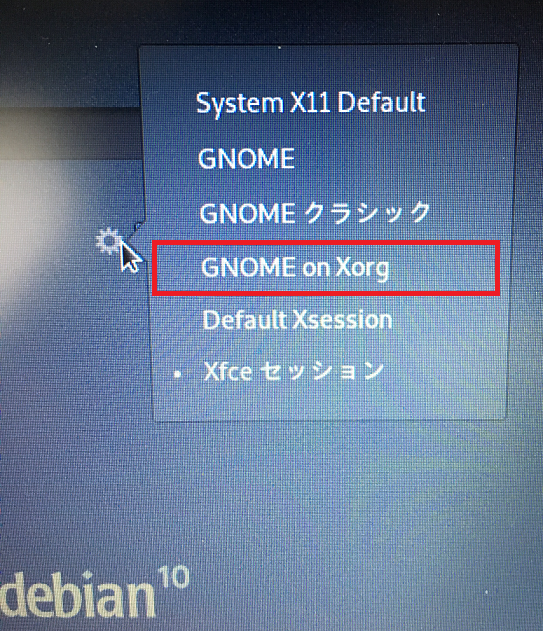
\includegraphics[width=0.5\hsize]{image201902/GDM_GNOME_select_mark.png}
\end{center}

\end{frame}


\begin{frame}{新機能:/usrマージ}

新規インストールは /usr マージした状態

\begin{itemize}
  \item /\{bin,sbin,lib\} は シンボリックリンク
\end{itemize}

\begin{table}[htb]
  \begin{tabular}{|ccc|}
    \hline
    /bin  & → & /usr/bin \\ \hline
    /sbin & → & /usr/sbin \\ \hline
    /lib  & → & /usr/lib \\
    \hline
  \end{tabular}
\end{table}

\begin{itemize}
\item Debian 以外から提供されるソフトウェアを利用している場合は要注意
\end{itemize}

\end{frame}


\begin{frame}{新機能:その他}% [containsverbatim]

\begin{itemize}
\item APTへのセキュリティ強化オプションの追加
\item stableポイントリリースに対する Unattended-upgrades の挙動
\item Cryptsetup の on-disk LUKS2 への変更
\item CUPS 2.2.10 でのドライバーレス印刷機能
\item Allwinner A64 ベースのデバイスでの基本機能サポート
\item など
\end{itemize}

\end{frame}


\begin{frame}{動作の変更や制約}% [containsverbatim]

\begin{itemize}
\item glibc が新しくなり、Linuxカーネルは 3.2 以上が必要
\item Debian 9 から PostgreSQL をアップグレードした場合は DB の再インデックス化が必要
\item Wayland で動作する GNOME の一部アプリケーションに不具合がある
  \begin{itemize}
  \item 例:synaptic、fcitx
  \item Wayland で動かない場合は Xorg で動かしてみてください
  \end{itemize}
\item phpmyadmin、redmine、virtualbox などのパッケージは未収録
\item python2.7 は非推奨
  \begin{itemize}
  \item Debian 11 では削除する方向で作業中
  \end{itemize}
\end{itemize}

\end{frame}


\begin{frame}{その他の変更や制約}% [containsverbatim]

\begin{itemize}
\item OpenSSL のデフォルトが TLS 1.2 と セキュリティレベル 2
\item ブラウザ、レンダリングエンジンは Firefox ESR、Chromium、webkit2gtk のみをセキュリティサポート
  \begin{itemize}
  \item webkit や khtml エンジンを使ったwebブラウザはセキュリティサポートされない
  \end{itemize}
\item Go 関連のパッケージは制限付きのセキュリティサポート
%\item gnome-disk-utility: LUKSパスワード変更でデータ消失の危険性
\item evolution-ews は パッケージから削除
  \begin{itemize}
  \item evolution で Exchange、Office365、Outlook にアクセスができなくなる
  \end{itemize}
\end{itemize}

\end{frame}


\subsection{バグレポート}

\begin{frame}{バグレポートをお願いします}% [containsverbatim]
  \begin{itemize}
  \item 何かおかしい動作や不具合を見つけた場合はバグレポートをお願いします
  \item バグレポートの例 \url{https://bugs.debian.org/cgi-bin/bugreport.cgi?bug=903529}
  \item バグレポートの仕方(レポートは英語で送る必要あり)
    \begin{itemize}
    \item \url{https://www.debian.org/Bugs/Reporting.ja.html}
    \end{itemize}
  \item バグレポートの前にちょっと相談してみたい方は、日本語のDebian JPメーリングリストや、SNSで相談してみてください
    \begin{itemize}
    \item \url{https://www.debian.or.jp/community/ml/openml.html}
    \item Twitter: @debian\_jp
    \end{itemize}
  \end{itemize}
\end{frame}

%-----------------------

\section{Debian Updates}

% 半年間の以下MLから抜粋して紹介する
%  debian-announce@lists.debian.org
%  debian-devel-announce@lists.debian.org

\begin{frame}
  \begin{center}\Huge{Debian Updates}\end{center}
\end{frame}


\subsection{released timeline}

\begin{frame}{Debian Updates}% [containsverbatim]

\begin{itemize}
\item 2019/04/27:  Updated Debian 9.9  released
\item 2019/07/06:  Debian 10 released
\item 2019/09/07:  Updated Debian 10.1 released
\item 2019/09/07:  Updated Debian 9.10 released
\item 2019/09/08:  Updated Debian 9.11 released
\item 2019/11/16:  Updated Debian 10.2 released
\end{itemize}

\end{frame}


\subsection{Bits from the DPL}

\begin{frame}{Debian Updates}% [containsverbatim]

Bits from the DPL

\begin{itemize}
\item 月に一度の Debian Project Leader である Sam さんのプロジェクトの進捗を報告
\item 時間のない方でもこれを読んでおけば Debian Project の大まかな動きがわかる
\end{itemize}

\small{
\begin{itemize}

%\item 2018/04/30 \url{https://lists.debian.org/debian-devel-announce/2019/04/msg00010.html}
%\item 2018/06/02 \url{https://lists.debian.org/debian-devel-announce/2019/06/msg00000.html}
\item 2018/07/02 \url{https://lists.debian.org/debian-devel-announce/2019/07/msg00000.html}
\item 2018/08/12 \url{https://lists.debian.org/debian-devel-announce/2019/08/msg00001.html}
\item 2019/09/18 \url{https://lists.debian.org/debian-devel-announce/2019/09/msg00001.html}
\item 2019/10/29 \url{https://lists.debian.org/debian-devel-announce/2019/10/msg00002.html}

\end{itemize}
}

\end{frame}


\subsection{Removal of the mips}

\begin{frame}{Debian Updates}% [containsverbatim]

2019/08/21: Removal of the mips architecture
  
\begin{itemize}
\item mips アーキテクチャ(32bit ビッグエンディアンのmips)を testing と unstable から削除
  \begin{itemize}
  \item mips を使っている場合は mipsel または mips64el へ移行を推奨 
  \end{itemize}
\item 次の Debian 11 では mips アーキテクチャはリリースされない
\item Debian 9 および Debian 10 では mips アーキテクチャのサポートは継続
\item サポート終了の理由
  \begin{itemize}
  \item 仮想アドレス空間が 2GB までという技術的な制限
  \item 開発する人や関心を持つ人の減少
  \end{itemize}
\item 参照:\url{https://lists.debian.org/debian-devel-announce/2019/08/msg00003.html}
\end{itemize}

\end{frame}


\subsection{Perl 5.30 transition}

\begin{frame}{Debian Updates}% [containsverbatim]

2019/10/05: Perl 5.30 transition underway
  
\begin{itemize}
\item unstable において perl パッケージを 5.30 への切替を実施
\item 【TIPS】
  \begin{itemize}
  \item  Debian においてプログラム言語やライブラリをバージョンアップすることを「トランジション」という
  \item トランジションを行うと依存するパッケージをすべてビルドしなおす大規模な処理が行われる
  \end{itemize}
\item 参照:\url{https://lists.debian.org/debian-devel-announce/2019/10/msg00000.html}
\end{itemize}

\end{frame}


\subsection{Python 2 removal}

\begin{frame}{Debian Updates}% [containsverbatim]

2019/11/02: Python 2 removal in sid/bullseye: Progress and next steps
  
\begin{itemize}
\item python 2 系列は2020年1月1日にサポート終了を迎えるとアナウンスされている
\item 次の Debian 11 では python 2.7 は削除する予定
\item 進捗状況の報告、バグ報告のタグ管理方法について案内が出ている
\item 参照:\url{https://lists.debian.org/debian-devel-announce/2019/11/msg00000.html}
\end{itemize}

\end{frame}


\subsection{Init Systems and systemd}

\begin{frame}{Debian Update}% [containsverbatim]

2019/11/17: General Resolution: Init Systems and systemd
2019/11/20: General Resolution: Init systems and systemd: new option

\begin{itemize}
\item 今後の Init System をどうするか投票する案内が出た
\item \url{https://www.debian.org/vote/2019/vote_002}
\item 選択肢は5つ
  \begin{itemize}
  \item Init deversity is Important and NMUable
  \item Systemd but we support exploring alternatives
  \item Focus on systemd for init system and other facilities
  \item Support non-systemd systems, without blocking progress
  \item Init diversity is Required
  \end{itemize}
\item 参照:\\
  \url{https://lists.debian.org/debian-devel-announce/2019/11/msg00001.html} \\
  \url{https://lists.debian.org/debian-devel-announce/2019/11/msg00002.html}
\end{itemize}

\end{frame}


%-----------------------

\section{日本語によるDebianの情報}

\begin{frame}\begin{center}\Huge{日本語によるDebianの情報}\end{center}\end{frame}

\begin{frame}{日本語によるDebianの情報}
\begin{itemize}
  \item Debian JP Project \\
      \url{https://www.debian.or.jp}
  \item 東京エリアDebian勉強会\\
      \url{https://tokyodebian-team.pages.debian.net/}
  \item 関西Debian勉強会 \\
      \url{https://wiki.debian.org/KansaiDebianMeeting}
  \item Twitter \\
      \url{@debian_jp}
  \item 雑誌 Software Design 技術評論社発行 \\
    「Debian Hot Topics」(隔月連載)
  \item 雑誌 シェルスクリプトマガジン USP研究所発行
\end{itemize}
\end{frame}

%----------------

\section{今後のイベント}

\begin{frame}\begin{center}\Huge{今後のイベント}\end{center}\end{frame}


\begin{frame}{今後のイベント}

\begin{itemize}
\item 11/24(日) 関西Debian勉強会
 \begin{itemize}
  \item \url{https://wiki.debian.org/KansaiDebianMeeting/20191124}
  \end{itemize}
\item 12/21(土)or 12/22(日) 東京エリアDebian勉強会(予定)
  \begin{itemize}
  \item \url{https://tokyodebian-team.pages.debian.net/2019-12.html}
  \item セミナー内容は調整中
  \end{itemize}
\end{itemize}

\end{frame}

%----------------

\end{document}

;;; Local Variables: ***
;;; outline-regexp: "\\([ 	]*\\\\\\(documentstyle\\|documentclass\\|emtext\\|section\\|begin{frame}\\)\\*?[ 	]*[[{]\\|[]+\\)" ***
;;; End: ***
